%%%%%%%%%%%%%%%%%%%%%%%%%%%%%%%%%%%%%%%%%
% Beamer Presentation
% LaTeX Template
% Version 1.0 (10/11/12)
%
% This template has been downloaded from:
% http://www.LaTeXTemplates.com
%
% License:% CC BY-NC-SA 3.0 (http://creativecommons.org/licenses/by-nc-sa/3.0/)
%
%%%%%%%%%%%%%%%%%%%%%%%%%%%%%%%%%%%%%%%%%

%----------------------------------------------------------------------------------------
%	PACKAGES AND THEMES
%----------------------------------------------------------------------------------------

\documentclass{beamer}

\mode<presentation> {

% The Beamer class comes with a number of default slide themes
% which change the colors and layouts of slides. Below this is a list
% of all the themes, uncomment each in turn to see what they look like.

%\usetheme{default}
%\usetheme{AnnArbor}
%\usetheme{Antibes}
%\usetheme{Bergen}
%\usetheme{Berkeley}
%\usetheme{Berlin}
%\usetheme{Boadilla}
%\usetheme{CambridgeUS}
%\usetheme{Copenhagen}
%\usetheme{Darmstadt}
%\usetheme{Dresden}
%\usetheme{Frankfurt}
%\usetheme{Goettingen}
%\usetheme{Hannover}
%\usetheme{Ilmenau}
%\usetheme{JuanLesPins}
%\usetheme{Luebeck}
\usetheme{Madrid}
%\usetheme{Malmoe}
%\usetheme{Marburg}
%\usetheme{Montpellier}
%\usetheme{PaloAlto}
%\usetheme{Pittsburgh}
%\usetheme{Rochester}
%\usetheme{Singapore}
%\usetheme{Szeged}
%\usetheme{Warsaw}

% As well as themes, the Beamer class has a number of color themes
% for any slide theme. Uncomment each of these in turn to see how it
% changes the colors of your current slide theme.

%\usecolortheme{albatross}
%\usecolortheme{beaver}
%\usecolortheme{beetle}
%\usecolortheme{crane}
%\usecolortheme{dolphin}
%\usecolortheme{dove}
%\usecolortheme{fly}
%\usecolortheme{lily}
%\usecolortheme{orchid}
%\usecolortheme{rose}
%\usecolortheme{seagull}
%\usecolortheme{seahorse}
%\usecolortheme{whale}
%\usecolortheme{wolverine}

%\setbeamertemplate{footline} % To remove the footer line in all slides uncomment this line
%\setbeamertemplate{footline}[page number] % To replace the footer line in all slides with a simple slide count uncomment this line

%\setbeamertemplate{navigation symbols}{} % To remove the navigation symbols from the bottom of all slides uncomment this line
}

\usepackage{graphicx} % Allows including images
\usepackage{booktabs} % Allows the use of \toprule, \midrule and \bottomrule in tables
\usepackage{color}
\usepackage{caption}
\usepackage{subcaption}
%----------------------------------------------------------------------------------------
%	TITLE PAGE
%----------------------------------------------------------------------------------------

\title[Thermal Conductivity]{A method for Computation of Thermal Conductivty} % The short title appears at the bottom of every slide, the full title is only on the title page

\author{Yerong Li} % Your name
\institute[NJU]{}% Your institution as it will appear on the bottom of every slide, may be shorthand to save space
\date{\today} % Date, can be changed to a custom date

\begin{document}

\begin{frame}
\titlepage % Print the title page as the first slide
\end{frame}

\begin{frame}
\frametitle{Overview} % Table of contents slide, comment this block out to remove it
\tableofcontents % Throughout your presentation, if you choose to use \section{} and \subsection{} commands, these will automatically be printed on this slide as an overview of your presentation
\end{frame}

%----------------------------------------------------------------------------------------
%	PRESENTATION SLIDES
%----------------------------------------------------------------------------------------
\section*{Introduction}
\begin{frame}
\frametitle{Introduction}
\begin{figure}
  \begin{subfigure}[b]{.45\linewidth}
    \centering
    %\caption{First subfigure}
    %\label{fig:a}
    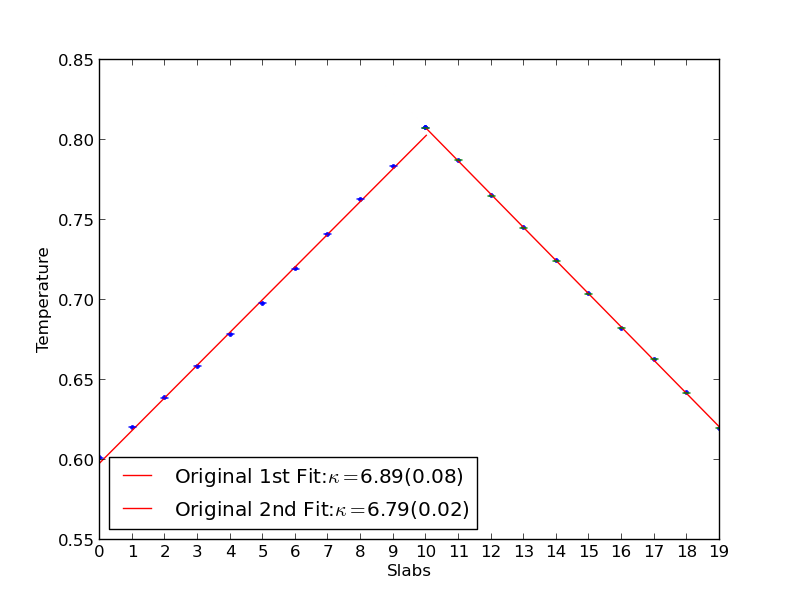
\includegraphics[height=4cm]{pf1.png}
  \end{subfigure}\hfill
  \begin{subfigure}[b]{.45\linewidth}
    \centering
    %\caption{Second subfigure}
    %\label{fig:b}
    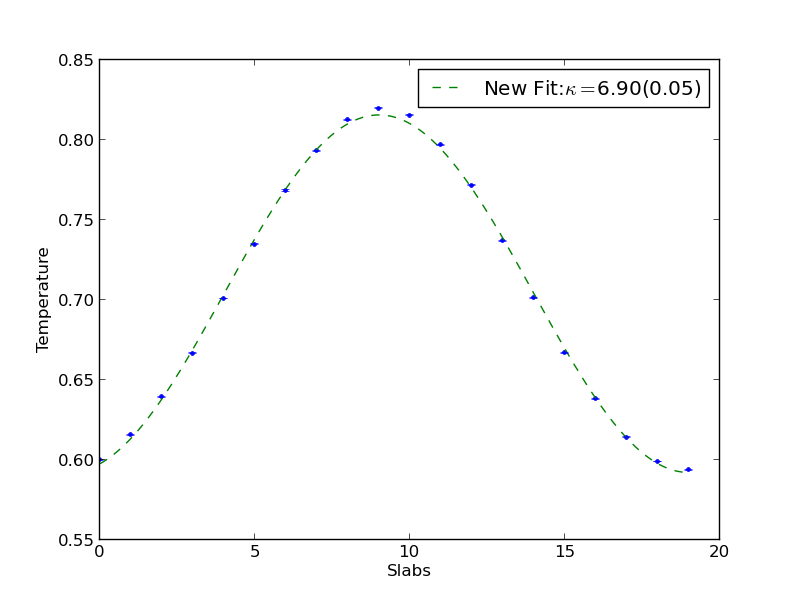
\includegraphics[height=4cm]{pf2.png}
  \end{subfigure}\hfill
%\caption{A figure}\label{fig:1}
\end{figure}
\end{frame}
%------------------------------------------------------------------------------
%\begin{frame}
%\begin{figure}[htb!]
%\begin{subfigure}
%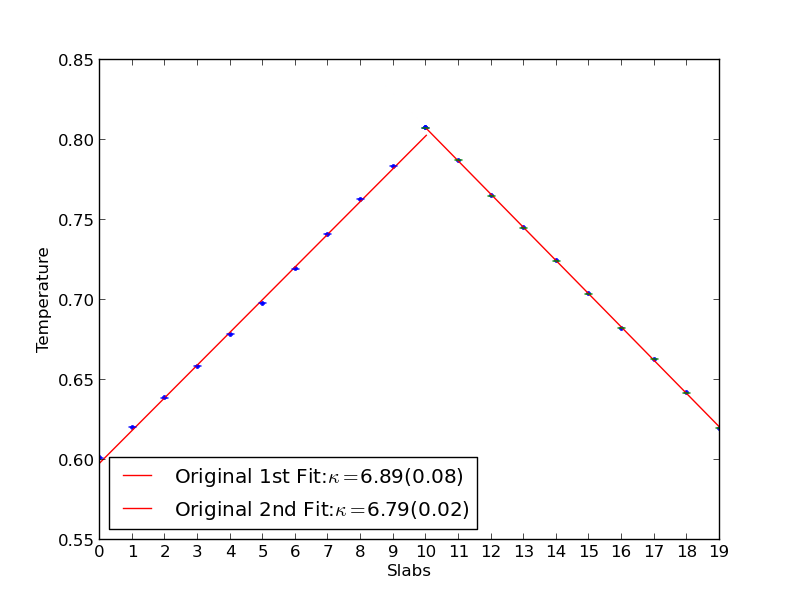
\includegraphics{pf1.png}
%\end{subfigure}\hfill
%\begin{subfigure}
%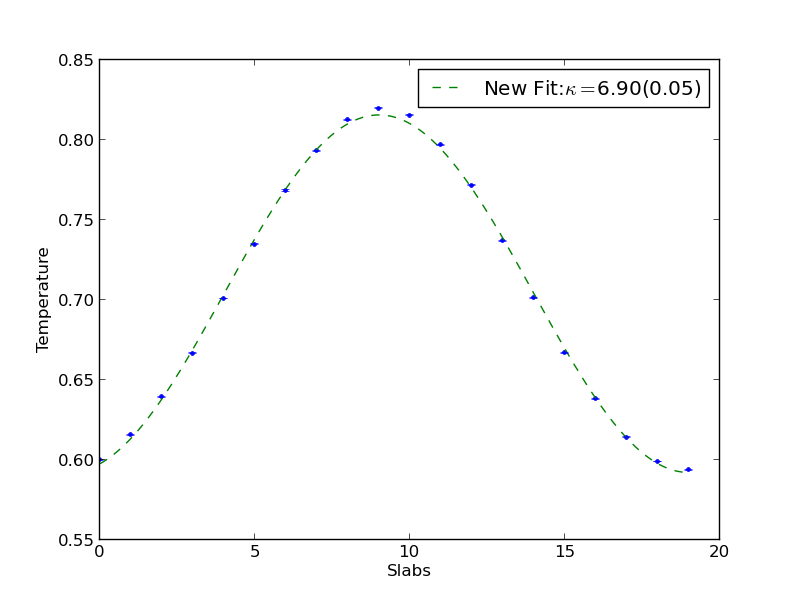
\includegraphics{pf2.png}
%\end{subfigure}\hfill
%\end{figure}[htb!]
%\end{frame}
%------------------------------------------------
\section{Theory} % Sections can be created in order to organize your presentation into discrete blocks, all sections and subsections are automatically printed in the table of contents as an overview of the talk
%------------------------------------------------

%ubsection{Subsection Example} % A subsection can be created just before a set of slides with a common theme to further break down your presentation into chunks

\begin{frame}
\frametitle{Theory}
\begin{equation*}
J_x(x)=\frac{1}{\Omega}\sum\limits_{Q} \hbar \omega v_{Qx}N_Q(x)
\end{equation*}
\begin{equation*}
J_x(q)=-\kappa(q)\nabla{T(q)} 
\end{equation*}
\begin{center}
$\Longrightarrow$
\end{center}
\begin{equation*}
\textcolor{red}{\kappa(q)=\frac{1}{\Omega}\sum\limits_{Q} \frac{\hbar \omega v_{Qx}^2(\partial n_Q / \partial T)}{1/\tau_Q +iqv_{Qx}}\nabla{T(q)}} \longrightarrow \textcolor{red}{q\rightarrow 0} 
\end{equation*}
\begin{center}
$\Longrightarrow$
\end{center}
\begin{equation*}
\kappa(x-x')=\frac{1}{\Omega}\sum\limits_{Q}^{v_{Qx}>0}\hbar \omega_{Qx}v_{Qx}e^{-\vert{x-x'}\vert{/}v_{Qx}\tau_{Q}}
\end{equation*}
%\begin{itemize}
%\item Aliquam blandit faucibus nisi, sit amet dapibus enim tempus eu
%\item Nulla commodo, erat quis gravida posuere, elit lacus lobortis est, quis porttitor odio mauris at libero
%\item Nam cursus est eget velit posuere pellentesque
%\item Vestibulum faucibus velit a augue condimentum quis convallis nulla gravida
%\end{itemize}
\end{frame}

%------------------------------------------------%------------------------------------------------
\section{Test on liquid}
%------------------------------------------------
%
%\begin{frame}
%\frametitle{Test on Liquid}
\begin{frame}
\frametitle{Test on Liquid}
\begin{figure}
  \begin{subfigure}[b]{.45\linewidth}
    \centering
    %\caption{First subfigure}
    %\label{fig:a}
    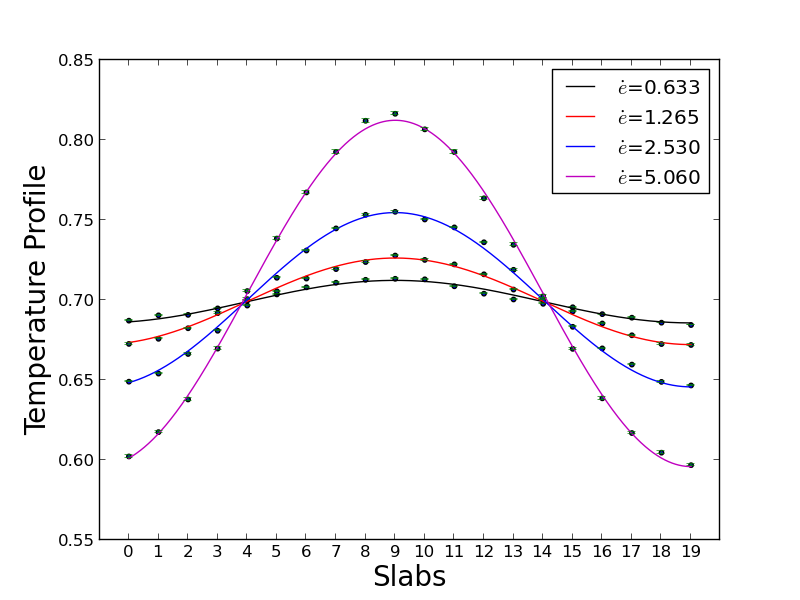
\includegraphics[height=4.5cm]{liquid.png}
  \end{subfigure}\hfill
  \begin{subfigure}[b]{.45\linewidth}
    \centering
    %\caption{Second subfigure}
    %\label{fig:b}
    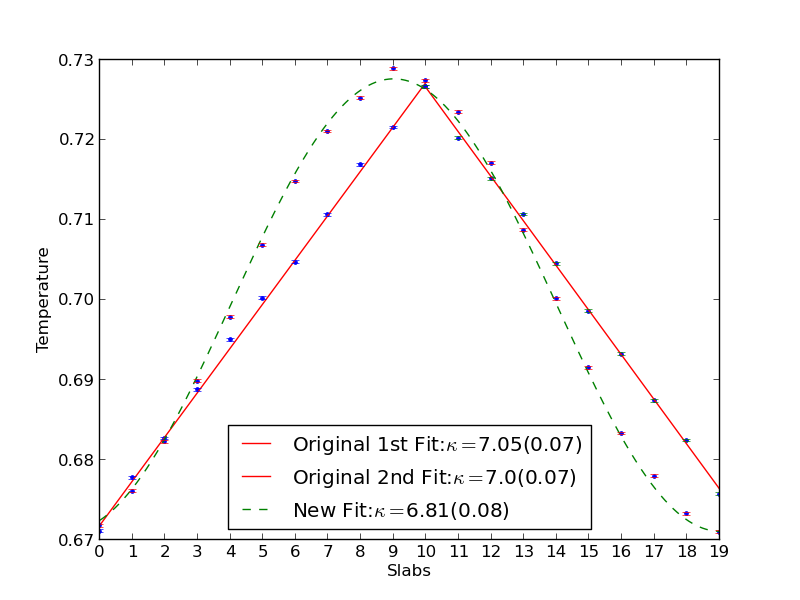
\includegraphics[height=4.5cm]{amplitude.png}
  \end{subfigure}\hfill
%\caption{A figure}\label{fig:1}
\end{figure}
\end{frame}
%\begin{figure}
%  \begin{subfigure}[b]{.45\linewidth}
%    \centering
    %\caption{First subfigure}
    %\label{fig:a}
%    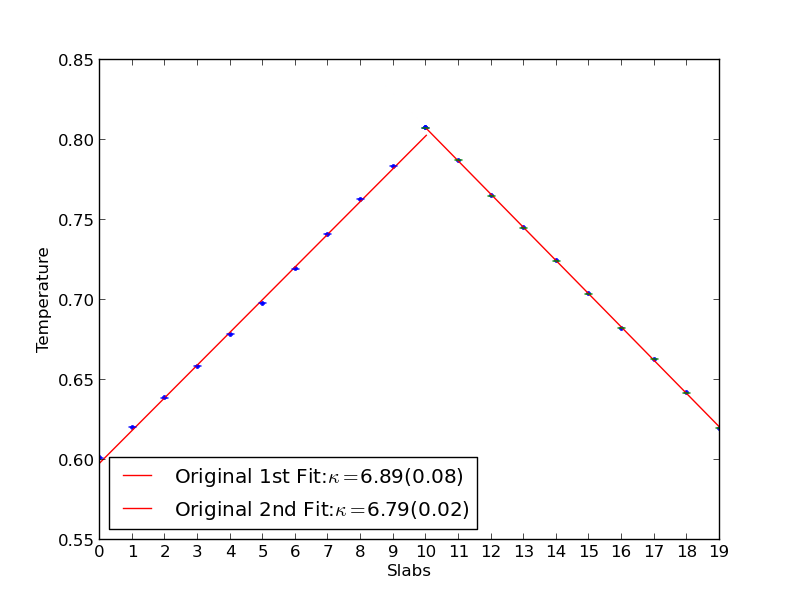
\includegraphics[height=4cm]{pf1.png}
%  \end{subfigure}\hfill
%  \begin{subfigure}[b]{.45\linewidth}
%    \centering
    %\caption{Second subfigure}
    %\label{fig:b}
%    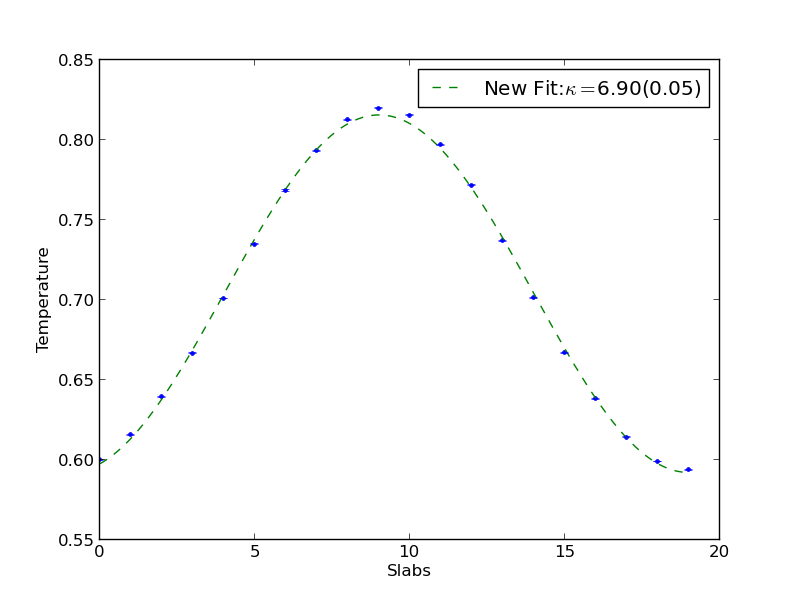
\includegraphics[height=4cm]{pf2.png}
%  \end{subfigure}\hfill
%\caption{A figure}\label{fig:1}
%\end{figure}
%------------------------------------------------
\begin{frame}
\begin{figure}
  \begin{subfigure}[b]{.45\linewidth}
    \centering
    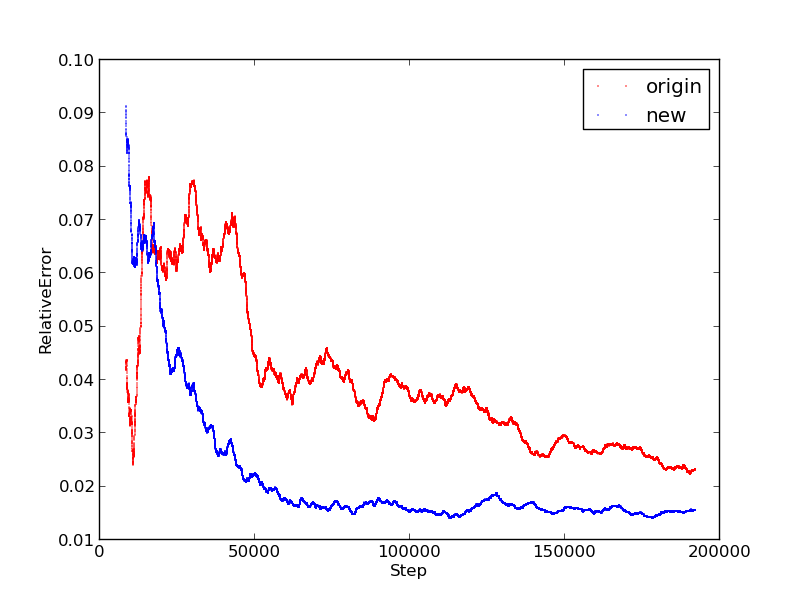
\includegraphics[height=4.5cm]{RelativeError.png}
  \end{subfigure}\hfill
  \begin{subfigure}[b]{.45\linewidth}
    \centering
    %\caption{Second subfigure}
    %\label{fig:b}
    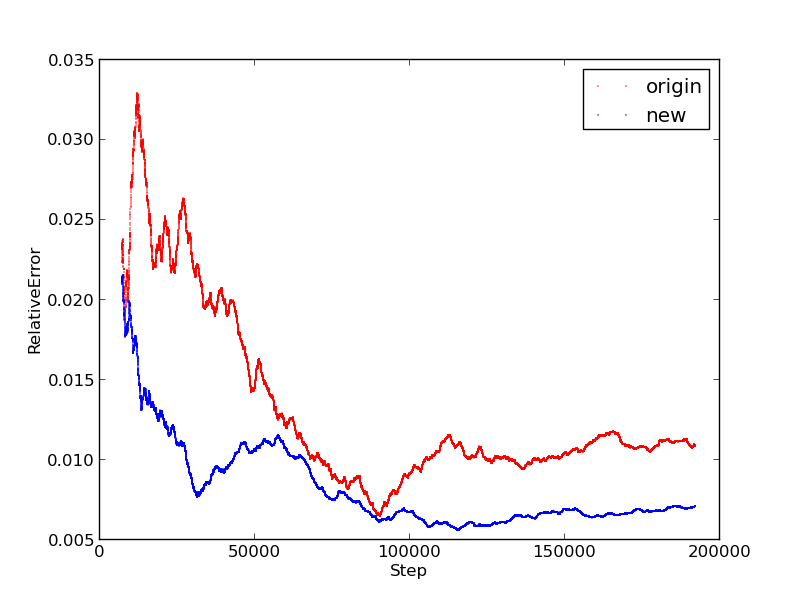
\includegraphics[height=4.5cm]{RelativeError2.png}
  \end{subfigure}\hfill
%\caption{A figure}\label{fig:1}
\end{figure}
\end{frame}

\section{Review on Theory}
\begin{frame}
\frametitle{Theory:Debye Model}
\begin{block}{$\kappa(q)$}
\begin{equation*}
\kappa(q)=\frac{1}{\Omega}\sum\limits_{Q}\hbar\omega\frac{\partial n_Q}{\partial T}v_{Qx}^2\tau_Q\times[\frac{1}{1+(qv_{Qx}\tau_Q)^2}]
\end{equation*}
\begin{equation*}
\vert v_Q\vert=v
\end{equation*}
\begin{equation*}
\tau_Q,\Lambda_Q\varpropto \left(\frac{\omega_{D}}{\omega}\right)^p ,p=0,1,2,3,4
\end{equation*}
\end{block}

\begin{block}{$\kappa_D$:Thermal Conduction in Debye Model}
\begin{equation*}
\kappa =\frac{1}{3}v\int_0^{\omega_D} {\Lambda}(\omega)c{\omega}d{\omega}=\frac{3}{3-p}\times \Lambda_{min}\times{C}_{\infty}
\end{equation*}
\end{block}
\end{frame}
\begin{frame}
\frametitle{Infinite Crystal}
\begin{figure}
    \centering
    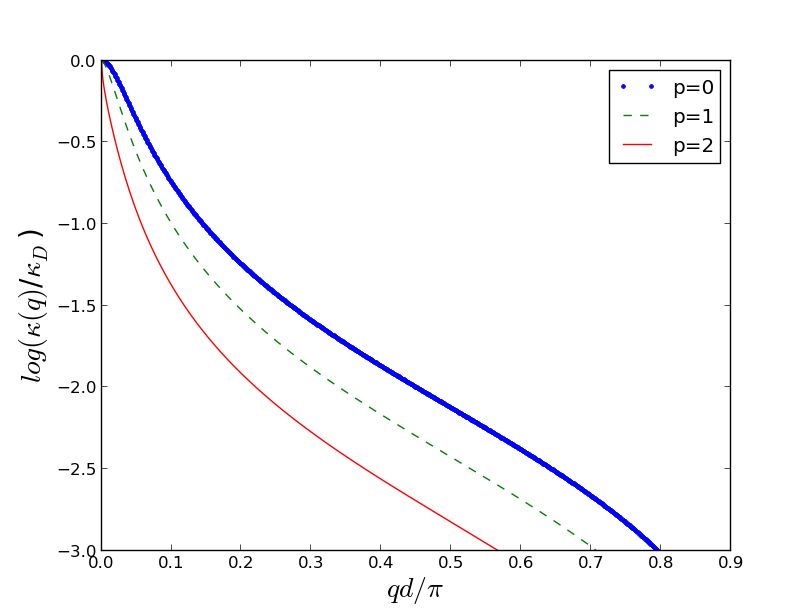
\includegraphics[height=8cm]{DebyeIn.png}
\end{figure}
\end{frame}

\begin{frame}
\frametitle{Finite Model}
\begin{figure}
    \centering
    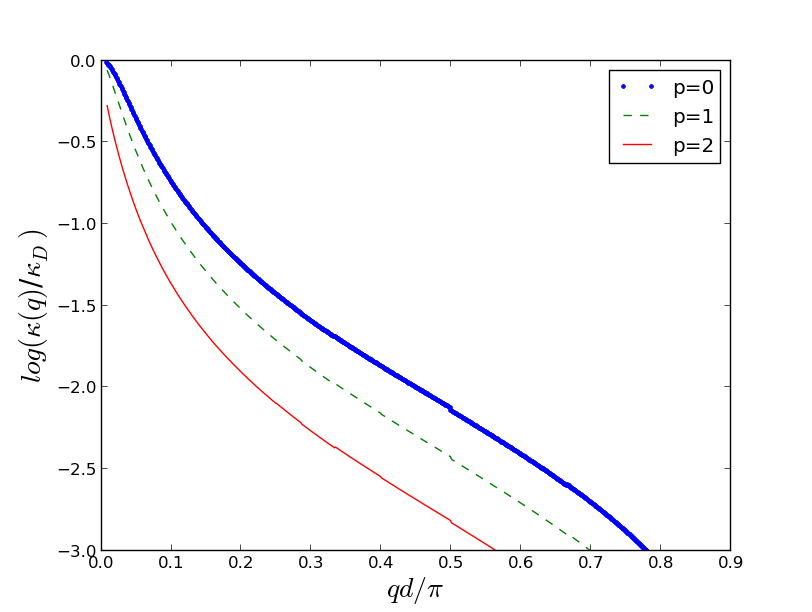
\includegraphics[height=8cm]{BZ.png}
\end{figure}
\end{frame}

\begin{frame}
\frametitle{Finite Model}
\centering
\begin{equation*}
\kappa(q)=\frac{1}{\Omega}\sum\limits_{Q}\hbar\omega\frac{\partial n_Q}{\partial T}v_{Qx}^2\tau_Q\times[\frac{1}{1+(qv_{Qx}\tau_Q)^2}]
\end{equation*}

Summing up in the 1st Brillouin Zone \\
\begin{center}
$\longrightarrow$ \\
$kappa(q) \rightarrow \kappa_D$
\end{center}
\end{frame}

\begin{frame}
\frametitle{Cross Section}
\begin{figure}
    \centering
    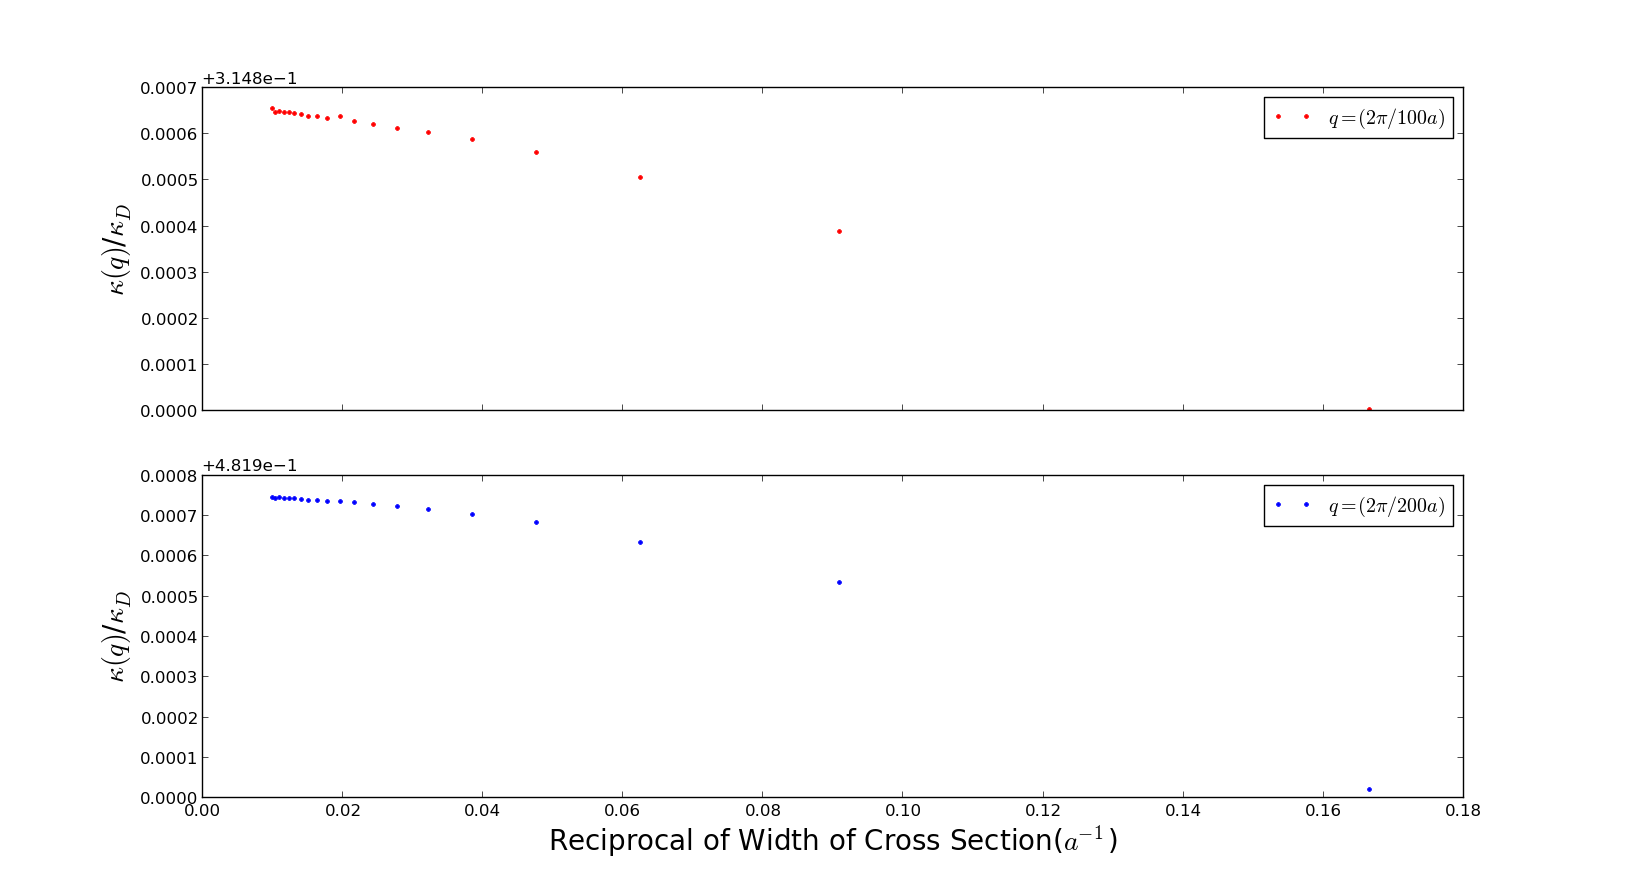
\includegraphics[height=6cm]{Cross.png}
\end{figure}
\end{frame}

\section{Test on Crystal}
\begin{frame}
\frametitle{Test on Crystal}
\begin{figure}
    \centering
    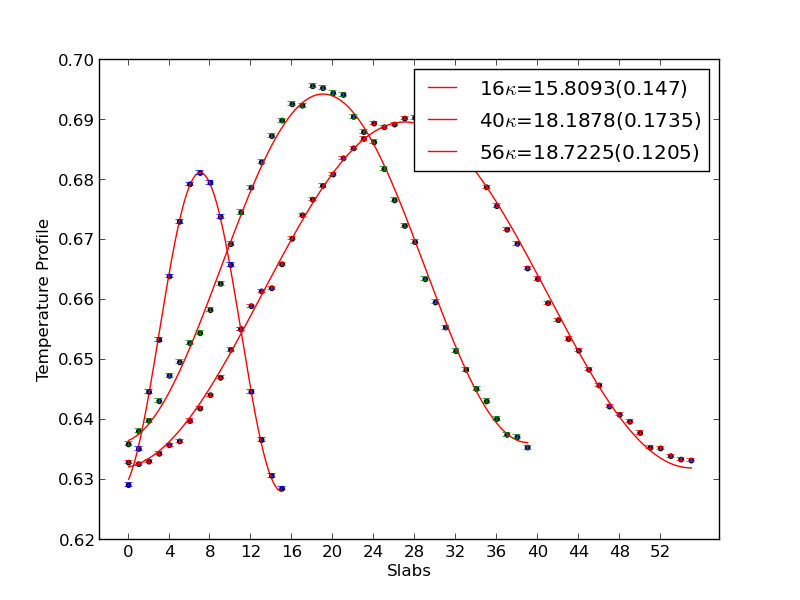
\includegraphics[height=8cm]{Experiments.png}
\end{figure}
\end{frame}
\begin{frame}
\frametitle{Test on Crystal}
\begin{figure}
    \centering
    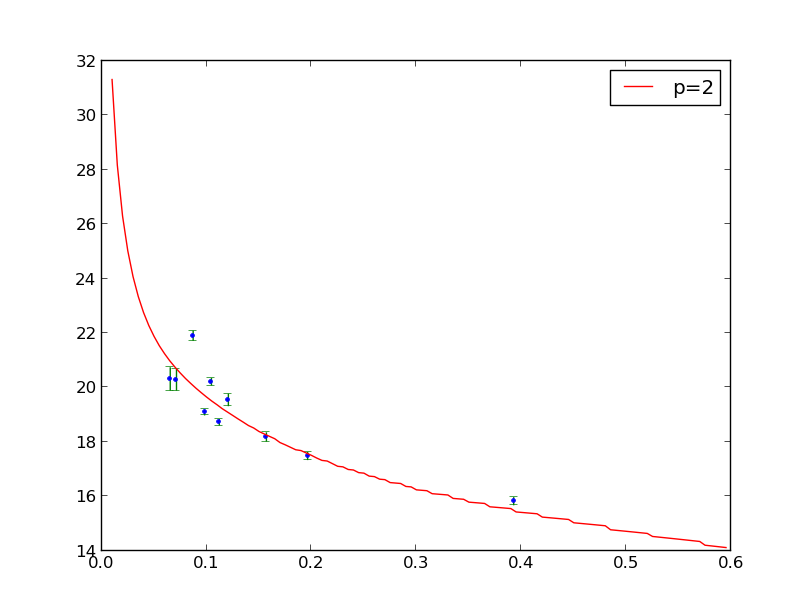
\includegraphics[height=8cm]{ConEx.png}
\end{figure}
\end{frame}

%------------------------------------------------
\section{Conclusion}
\begin{frame}
\frametitle{Conclusion}
\begin{block}{Conclusion 1}
The sine temperature profile converges faster than the simple input at two ends.
\end{block}

\begin{block}{Conclusion 2}
The treatment of solution from PBE does not need very large cross section.
\end{block}

\begin{block}{Conclusion 3}
This method of extrapolation is expected to give a reasonable result.
\end{block}
\end{frame}


%\begin{frame}[fragile] % Need to use the fragile option when verbatim is used in the slide
%\frametitle{Citation}
%An example of the \verb|\cite| command to cite within the presentation:\\~

%This statement requires citation \cite{p1}.
%\end{frame}

%------------------------------------------------

%\begin{frame}
%\frametitle{References}
%\footnotesize{
%\begin{thebibliography}{99} % Beamer does not support BibTeX so references must be inserted manually as %below
%\bibitem[Smith, 2012]{p1} John Smith (2012)
%\newblock Title of the publication
%\newblock \emph{Journal Name} 12(3), 45 -- 678.
%\end{thebibliography}
%}
%\end{frame}
%
%------------------------------------------------

\begin{frame}
\Huge{\centerline{The End}}
\end{frame}

%----------------------------------------------------------------------------------------

\end{document} 
